\documentclass[tikz,border=2pt]{standalone}
\pdfmapfile{+cm.map}
\usepackage{pgfplots}
\pgfplotsset{compat=1.18}
\usetikzlibrary{arrows.meta}
\definecolor{ink}{HTML}{202B30}
\definecolor{red}{HTML}{971D2C}
\definecolor{soft}{HTML}{F4E9EB}
\definecolor{gray}{HTML}{51636D}
\definecolor{line}{HTML}{D6DDE0}
\definecolor{pale}{HTML}{F0F3F4}
\begin{document}
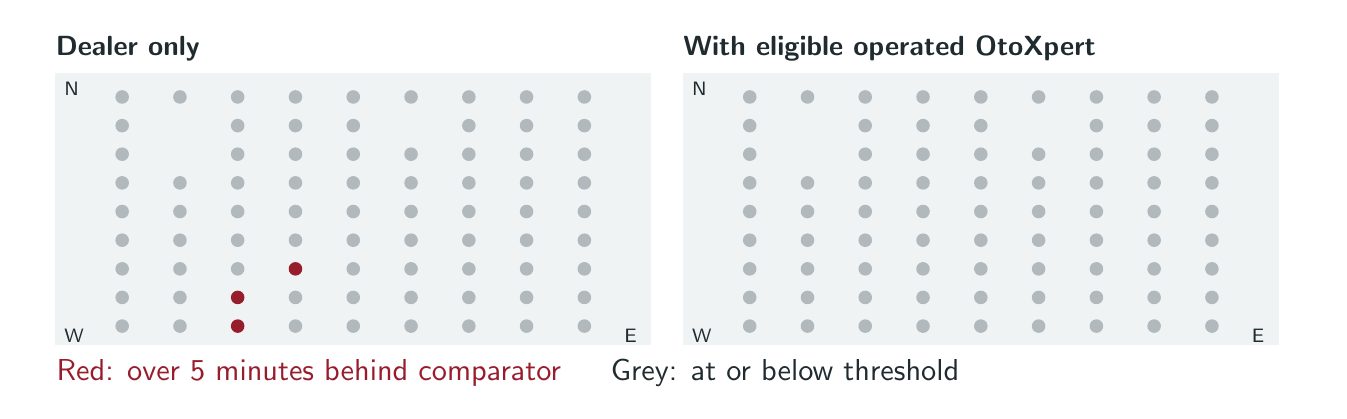
\begin{tikzpicture}[x=1cm,y=1cm,font=\sffamily\fontsize{10.5}{12}\selectfont,text=ink,arr/.style={-{Stealth[length=2mm]},draw=gray,thick}]
\path[use as bounding box] (0,0) rectangle (16.4,4.61);
\node[anchor=west,inner sep=0pt,font=\sffamily\bfseries] at (0.35,4.35) {Dealer only};
\fill[pale] (0.35,0.58) rectangle (7.92,4.03);
\fill[gray!45] (1.200,0.820) circle (2.45pt);\fill[gray!45] (1.934,0.820) circle (2.45pt);\fill[red] (2.667,0.820) circle (2.45pt);\fill[gray!45] (3.401,0.820) circle (2.45pt);\fill[gray!45] (4.135,0.820) circle (2.45pt);\fill[gray!45] (4.869,0.820) circle (2.45pt);\fill[gray!45] (5.603,0.820) circle (2.45pt);\fill[gray!45] (6.336,0.820) circle (2.45pt);\fill[gray!45] (7.070,0.820) circle (2.45pt);\fill[gray!45] (1.200,1.184) circle (2.45pt);\fill[gray!45] (1.934,1.184) circle (2.45pt);\fill[red] (2.667,1.184) circle (2.45pt);\fill[gray!45] (3.401,1.184) circle (2.45pt);\fill[gray!45] (4.135,1.184) circle (2.45pt);\fill[gray!45] (4.869,1.184) circle (2.45pt);\fill[gray!45] (5.603,1.184) circle (2.45pt);\fill[gray!45] (6.336,1.184) circle (2.45pt);\fill[gray!45] (7.070,1.184) circle (2.45pt);\fill[gray!45] (1.200,1.547) circle (2.45pt);\fill[gray!45] (1.934,1.547) circle (2.45pt);\fill[gray!45] (2.667,1.547) circle (2.45pt);\fill[red] (3.401,1.547) circle (2.45pt);\fill[gray!45] (4.135,1.547) circle (2.45pt);\fill[gray!45] (4.869,1.547) circle (2.45pt);\fill[gray!45] (5.603,1.547) circle (2.45pt);\fill[gray!45] (6.336,1.547) circle (2.45pt);\fill[gray!45] (7.070,1.547) circle (2.45pt);\fill[gray!45] (1.200,1.911) circle (2.45pt);\fill[gray!45] (1.934,1.911) circle (2.45pt);\fill[gray!45] (2.667,1.911) circle (2.45pt);\fill[gray!45] (3.401,1.911) circle (2.45pt);\fill[gray!45] (4.135,1.911) circle (2.45pt);\fill[gray!45] (4.869,1.911) circle (2.45pt);\fill[gray!45] (5.603,1.911) circle (2.45pt);\fill[gray!45] (6.336,1.911) circle (2.45pt);\fill[gray!45] (7.070,1.911) circle (2.45pt);\fill[gray!45] (1.200,2.275) circle (2.45pt);\fill[gray!45] (1.934,2.275) circle (2.45pt);\fill[gray!45] (2.667,2.275) circle (2.45pt);\fill[gray!45] (3.401,2.275) circle (2.45pt);\fill[gray!45] (4.135,2.275) circle (2.45pt);\fill[gray!45] (4.869,2.275) circle (2.45pt);\fill[gray!45] (5.603,2.275) circle (2.45pt);\fill[gray!45] (6.336,2.275) circle (2.45pt);\fill[gray!45] (7.070,2.275) circle (2.45pt);\fill[gray!45] (1.200,2.639) circle (2.45pt);\fill[gray!45] (1.934,2.639) circle (2.45pt);\fill[gray!45] (2.667,2.639) circle (2.45pt);\fill[gray!45] (3.401,2.639) circle (2.45pt);\fill[gray!45] (4.135,2.639) circle (2.45pt);\fill[gray!45] (4.869,2.639) circle (2.45pt);\fill[gray!45] (5.603,2.639) circle (2.45pt);\fill[gray!45] (6.336,2.639) circle (2.45pt);\fill[gray!45] (7.070,2.639) circle (2.45pt);\fill[gray!45] (1.200,3.003) circle (2.45pt);\fill[gray!45] (2.667,3.003) circle (2.45pt);\fill[gray!45] (3.401,3.003) circle (2.45pt);\fill[gray!45] (4.135,3.003) circle (2.45pt);\fill[gray!45] (4.869,3.003) circle (2.45pt);\fill[gray!45] (5.603,3.003) circle (2.45pt);\fill[gray!45] (6.336,3.003) circle (2.45pt);\fill[gray!45] (7.070,3.003) circle (2.45pt);\fill[gray!45] (1.200,3.366) circle (2.45pt);\fill[gray!45] (2.667,3.366) circle (2.45pt);\fill[gray!45] (3.401,3.366) circle (2.45pt);\fill[gray!45] (4.135,3.366) circle (2.45pt);\fill[gray!45] (5.603,3.366) circle (2.45pt);\fill[gray!45] (6.336,3.366) circle (2.45pt);\fill[gray!45] (7.070,3.366) circle (2.45pt);\fill[gray!45] (1.200,3.730) circle (2.45pt);\fill[gray!45] (1.934,3.730) circle (2.45pt);\fill[gray!45] (2.667,3.730) circle (2.45pt);\fill[gray!45] (3.401,3.730) circle (2.45pt);\fill[gray!45] (4.135,3.730) circle (2.45pt);\fill[gray!45] (4.869,3.730) circle (2.45pt);\fill[gray!45] (5.603,3.730) circle (2.45pt);\fill[gray!45] (6.336,3.730) circle (2.45pt);\fill[gray!45] (7.070,3.730) circle (2.45pt);\node[anchor=west,inner sep=0pt,font=\sffamily\scriptsize] at (0.45999999999999996,0.7) {W};
\node[anchor=west,inner sep=0pt,font=\sffamily\scriptsize] at (7.569999999999999,0.7) {E};
\node[anchor=west,inner sep=0pt,font=\sffamily\scriptsize] at (0.45999999999999996,3.83) {N};
\node[anchor=west,inner sep=0pt,font=\sffamily\bfseries] at (8.32,4.35) {With eligible operated OtoXpert};
\fill[pale] (8.32,0.58) rectangle (15.89,4.03);
\fill[gray!45] (9.170,0.820) circle (2.45pt);\fill[gray!45] (9.904,0.820) circle (2.45pt);\fill[gray!45] (10.637,0.820) circle (2.45pt);\fill[gray!45] (11.371,0.820) circle (2.45pt);\fill[gray!45] (12.105,0.820) circle (2.45pt);\fill[gray!45] (12.839,0.820) circle (2.45pt);\fill[gray!45] (13.573,0.820) circle (2.45pt);\fill[gray!45] (14.306,0.820) circle (2.45pt);\fill[gray!45] (15.040,0.820) circle (2.45pt);\fill[gray!45] (9.170,1.184) circle (2.45pt);\fill[gray!45] (9.904,1.184) circle (2.45pt);\fill[gray!45] (10.637,1.184) circle (2.45pt);\fill[gray!45] (11.371,1.184) circle (2.45pt);\fill[gray!45] (12.105,1.184) circle (2.45pt);\fill[gray!45] (12.839,1.184) circle (2.45pt);\fill[gray!45] (13.573,1.184) circle (2.45pt);\fill[gray!45] (14.306,1.184) circle (2.45pt);\fill[gray!45] (15.040,1.184) circle (2.45pt);\fill[gray!45] (9.170,1.547) circle (2.45pt);\fill[gray!45] (9.904,1.547) circle (2.45pt);\fill[gray!45] (10.637,1.547) circle (2.45pt);\fill[gray!45] (11.371,1.547) circle (2.45pt);\fill[gray!45] (12.105,1.547) circle (2.45pt);\fill[gray!45] (12.839,1.547) circle (2.45pt);\fill[gray!45] (13.573,1.547) circle (2.45pt);\fill[gray!45] (14.306,1.547) circle (2.45pt);\fill[gray!45] (15.040,1.547) circle (2.45pt);\fill[gray!45] (9.170,1.911) circle (2.45pt);\fill[gray!45] (9.904,1.911) circle (2.45pt);\fill[gray!45] (10.637,1.911) circle (2.45pt);\fill[gray!45] (11.371,1.911) circle (2.45pt);\fill[gray!45] (12.105,1.911) circle (2.45pt);\fill[gray!45] (12.839,1.911) circle (2.45pt);\fill[gray!45] (13.573,1.911) circle (2.45pt);\fill[gray!45] (14.306,1.911) circle (2.45pt);\fill[gray!45] (15.040,1.911) circle (2.45pt);\fill[gray!45] (9.170,2.275) circle (2.45pt);\fill[gray!45] (9.904,2.275) circle (2.45pt);\fill[gray!45] (10.637,2.275) circle (2.45pt);\fill[gray!45] (11.371,2.275) circle (2.45pt);\fill[gray!45] (12.105,2.275) circle (2.45pt);\fill[gray!45] (12.839,2.275) circle (2.45pt);\fill[gray!45] (13.573,2.275) circle (2.45pt);\fill[gray!45] (14.306,2.275) circle (2.45pt);\fill[gray!45] (15.040,2.275) circle (2.45pt);\fill[gray!45] (9.170,2.639) circle (2.45pt);\fill[gray!45] (9.904,2.639) circle (2.45pt);\fill[gray!45] (10.637,2.639) circle (2.45pt);\fill[gray!45] (11.371,2.639) circle (2.45pt);\fill[gray!45] (12.105,2.639) circle (2.45pt);\fill[gray!45] (12.839,2.639) circle (2.45pt);\fill[gray!45] (13.573,2.639) circle (2.45pt);\fill[gray!45] (14.306,2.639) circle (2.45pt);\fill[gray!45] (15.040,2.639) circle (2.45pt);\fill[gray!45] (9.170,3.003) circle (2.45pt);\fill[gray!45] (10.637,3.003) circle (2.45pt);\fill[gray!45] (11.371,3.003) circle (2.45pt);\fill[gray!45] (12.105,3.003) circle (2.45pt);\fill[gray!45] (12.839,3.003) circle (2.45pt);\fill[gray!45] (13.573,3.003) circle (2.45pt);\fill[gray!45] (14.306,3.003) circle (2.45pt);\fill[gray!45] (15.040,3.003) circle (2.45pt);\fill[gray!45] (9.170,3.366) circle (2.45pt);\fill[gray!45] (10.637,3.366) circle (2.45pt);\fill[gray!45] (11.371,3.366) circle (2.45pt);\fill[gray!45] (12.105,3.366) circle (2.45pt);\fill[gray!45] (13.573,3.366) circle (2.45pt);\fill[gray!45] (14.306,3.366) circle (2.45pt);\fill[gray!45] (15.040,3.366) circle (2.45pt);\fill[gray!45] (9.170,3.730) circle (2.45pt);\fill[gray!45] (9.904,3.730) circle (2.45pt);\fill[gray!45] (10.637,3.730) circle (2.45pt);\fill[gray!45] (11.371,3.730) circle (2.45pt);\fill[gray!45] (12.105,3.730) circle (2.45pt);\fill[gray!45] (12.839,3.730) circle (2.45pt);\fill[gray!45] (13.573,3.730) circle (2.45pt);\fill[gray!45] (14.306,3.730) circle (2.45pt);\fill[gray!45] (15.040,3.730) circle (2.45pt);\node[anchor=west,inner sep=0pt,font=\sffamily\scriptsize] at (8.43,0.7) {W};
\node[anchor=west,inner sep=0pt,font=\sffamily\scriptsize] at (15.54,0.7) {E};
\node[anchor=west,inner sep=0pt,font=\sffamily\scriptsize] at (8.43,3.83) {N};
\node[anchor=west,inner sep=0pt,text=red] at (0.36,0.23) {Red: over 5 minutes behind comparator};
\node[anchor=west,inner sep=0pt,] at (7.4,0.23) {Grey: at or below threshold};
\end{tikzpicture}\end{document}